\chapter{Business Intelligence}


\begin{description}
    \item[\Acl{bi}] \marginnote{\Acl{bi}}
        Transform raw data into information.
        Deliver the right information to the right people at the right time through the right channel.

    \item[\Ac{dwh}] \marginnote{\Acl{dwh}}
        Optimized repository that stores information for decision making processes.
        \Acp{dwh} are a specific type of \ac{dss}.

        Features:
        \begin{itemize}
            \item Subject-oriented: focused on enterprise specific concepts.
            \item Integrates data from different sources and provides an unified view.
            \item Non-volatile storage with change tracking. 
        \end{itemize}

    \item[\Ac{dm}] \marginnote{\Acl{dm}}
        Subset of the primary \ac{dwh} with information relevant to a specific business area.
\end{description}



\section{\Acl{olap} (\Ac{olap})}

\begin{description}
    \item[\ac{olap} analyses] \marginnote{\Acl{olap} (\Ac{olap})}
        Interactively navigate the information in a data warehouse.
        Allows to visualize different levels of aggregation.

    \item[\ac{olap} session] 
        Navigation path created by the operations of a user.
\end{description}

\begin{figure}[ht]
    \centering
    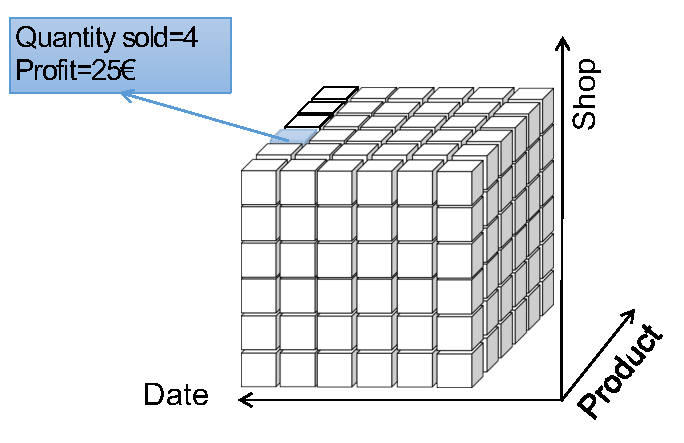
\includegraphics[width=0.35\textwidth]{img/_olap_cube.pdf}
    \caption{\ac{olap} data cube}
\end{figure}


\subsection{Operators}

\begin{description}
    \item[Roll-up] \marginnote{Roll-up}
        Increases the level of aggregation (i.e. \texttt{GROUP BY} in SQL). Some details are collapsed together.

    \item[Drill-down] \marginnote{Drill-down}
        Reduces the level of aggregation. Some details are reintroduced.
    
    \item[Slide-and-dice] \marginnote{Slide-and-dice}
        The slice operator reduces the number of dimensions (i.e. drops columns).

        The dice operator reduces the number of data being analyzed (i.e. \texttt{LIMIT} in SQL).

    \item[Pivot] \marginnote{Pivot}
        Changes the layout of the data to analyze it from a different viewpoint.

    \item[Drill-across] \marginnote{Drill-across}
        Links concepts from different data sources (i.e. \texttt{JOIN} in SQL).

    \item[Drill-through] \marginnote{Drill-through}
        Switches from multidimensional aggregated data to operational data (e.g. a spreadsheet).
\end{description}

\begin{figure}[ht]
    \begin{subfigure}{.33\textwidth}
        \centering
        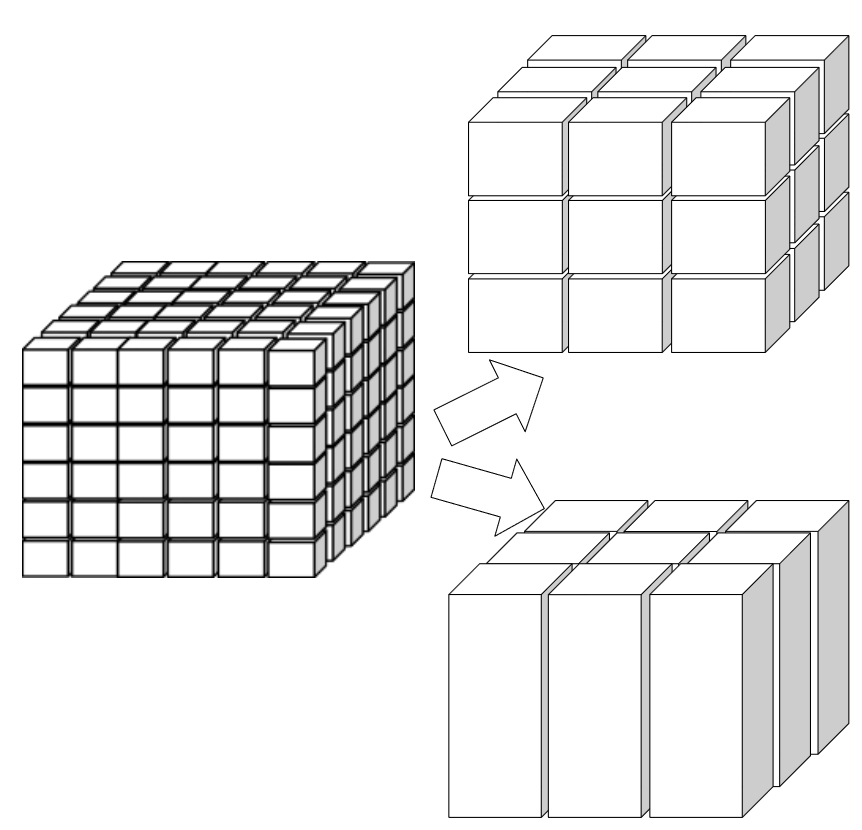
\includegraphics[width=.60\linewidth]{img/olap_rollup.png}
        \caption{\ac{olap} roll-up}
    \end{subfigure}%
    \begin{subfigure}{.33\textwidth}
        \centering
        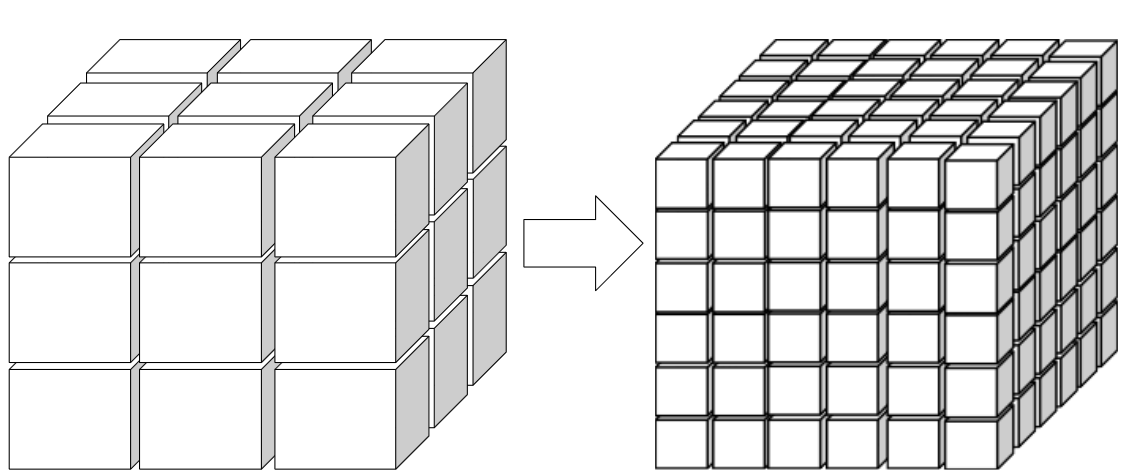
\includegraphics[width=.60\linewidth]{img/olap_drilldown.png}
        \caption{\ac{olap} drill-down}
    \end{subfigure}
    \begin{subfigure}{.33\textwidth}
        \centering
        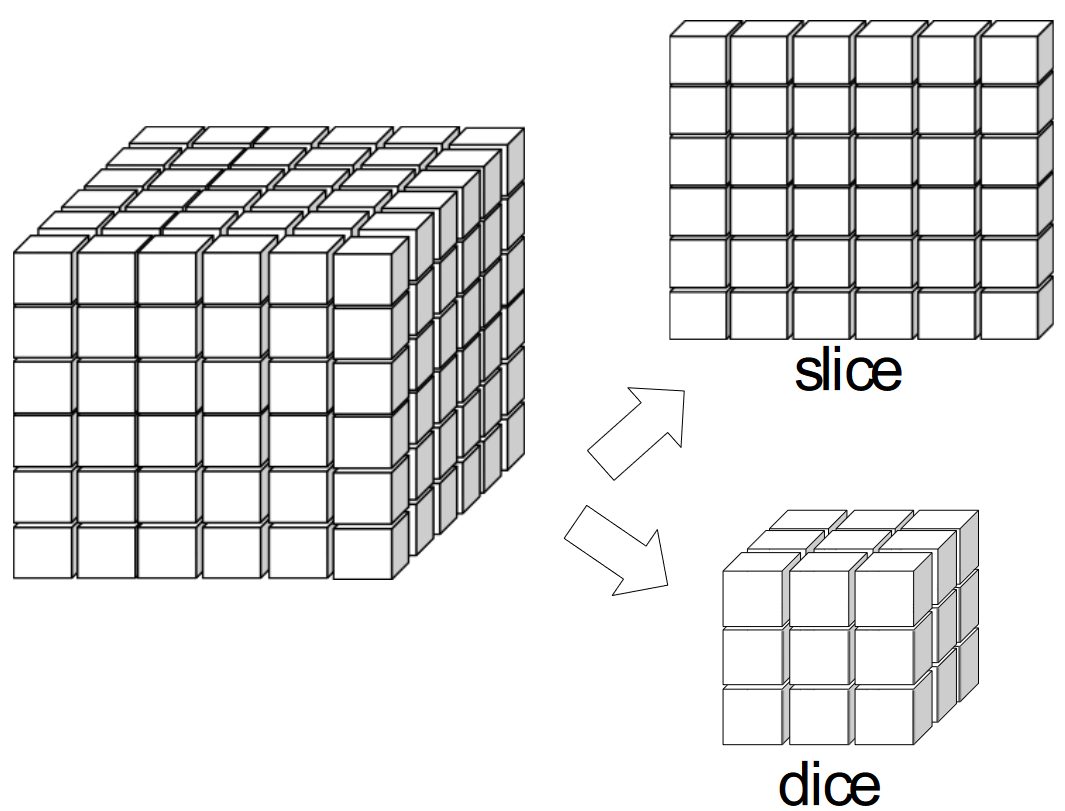
\includegraphics[width=.80\linewidth]{img/olap_slicedice.png}
        \caption{\ac{olap} slide-and-dice}
    \end{subfigure}
    \\
    \begin{subfigure}{.5\textwidth}
        \centering
        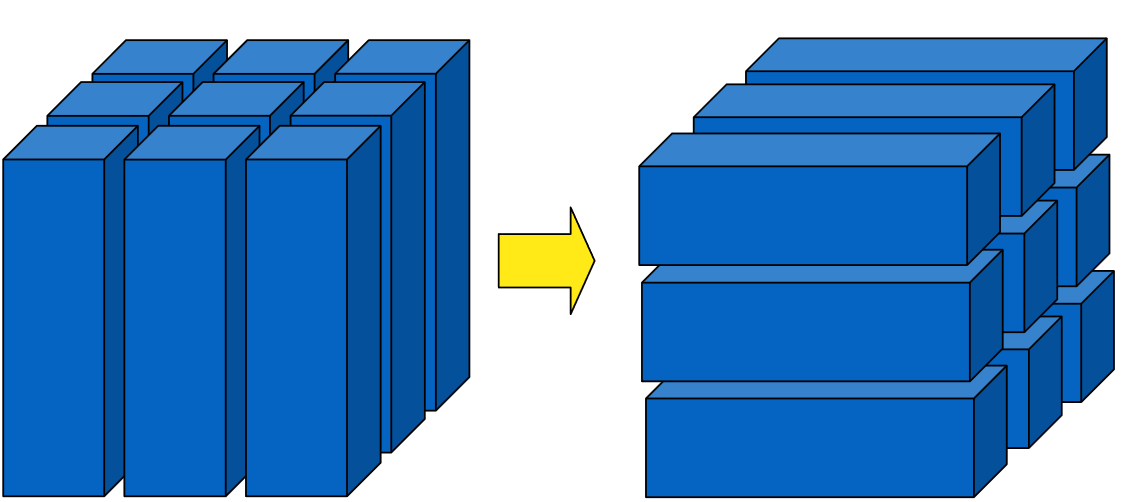
\includegraphics[width=.35\linewidth]{img/olap_pivot.png}
        \caption{\ac{olap} pivot}
    \end{subfigure}
    \begin{subfigure}{.5\textwidth}
        \centering
        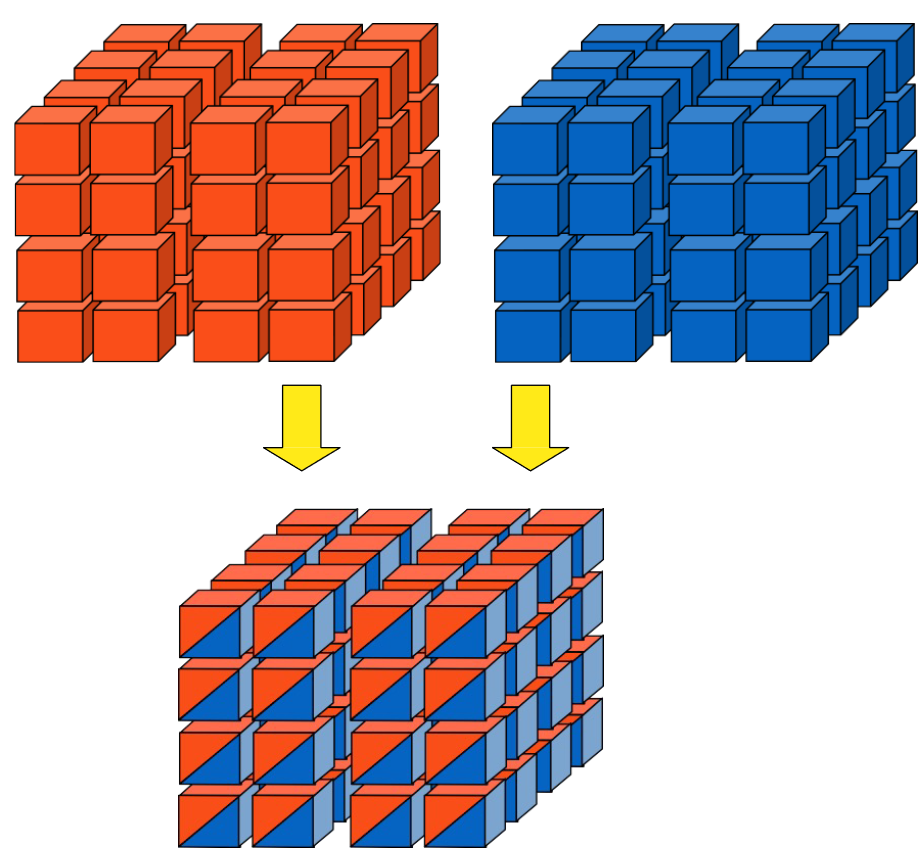
\includegraphics[width=.35\linewidth]{img/olap_drillacross.png}
        \caption{\ac{olap} drill-across}
    \end{subfigure}
    \\
    \begin{subfigure}{\textwidth}
        \centering
        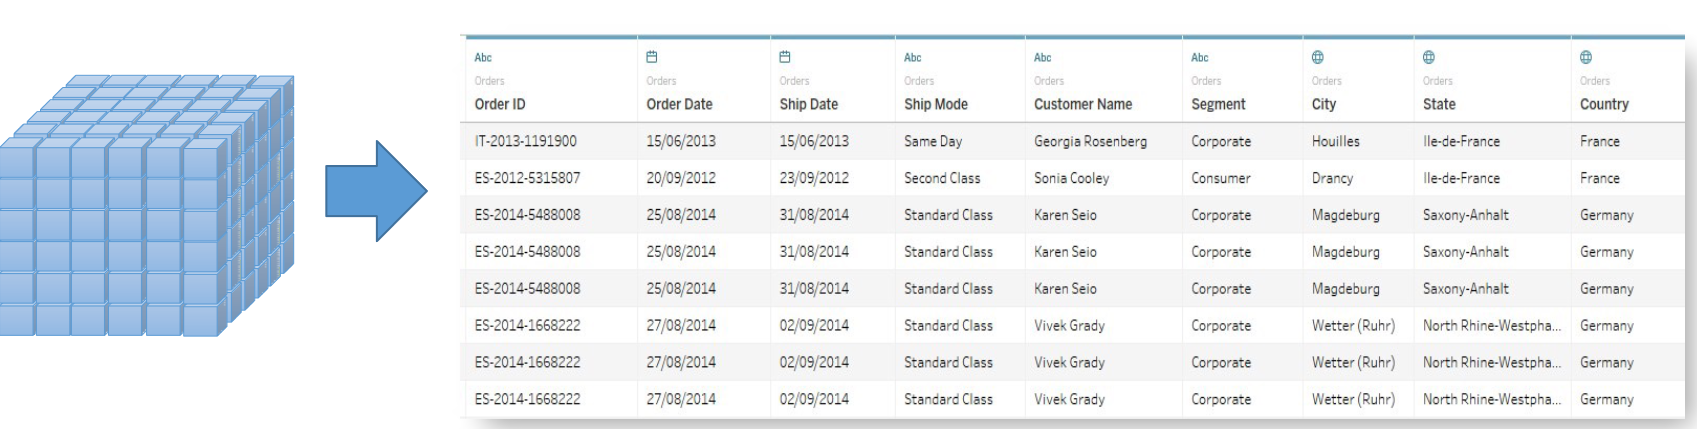
\includegraphics[width=.60\linewidth]{img/olap_drillthrough.png}
        \caption{\ac{olap} drill-through}
    \end{subfigure}
\end{figure}



\section{\Acl{etl} (\Ac{etl})}
\marginnote{\Acl{etl} (\Ac{etl})}
The \Ac{etl} process extracts, integrates and cleans operational data that will be loaded into a data warehouse.


\subsection{Extraction}

Extracted operational data can be:
\begin{descriptionlist}
    \item[Structured] \marginnote{Strucured data}
        with a predefined data model (e.g. relational DB, CSV)

    \item[Untructured] \marginnote{Unstrucured data}
        without a predefined data model (e.g. social media content)
\end{descriptionlist}

Extraction can be of two types:
\begin{descriptionlist}
    \item[Static] \marginnote{Static extraction}
        The entirety of the operational data are extracted to populate the
        data warehouse for the first time.
    
    \item[Incremental] \marginnote{Incremental extraction}
        Only changes applied since the last extraction are considered.
        Can be based on a timestamp or a trigger.
\end{descriptionlist}


\subsection{Cleaning}

Operational data may contain:
\begin{descriptionlist}
    \item[Duplicate data] 
    \item[Missing data] 
    \item[Improper use of fields] (e.g. saving the phone number in the \texttt{notes} field)
    \item[Wrong values] (e.g. 30th of February)
    \item[Inconsistency] (e.g. use of different abbreviations)
    \item[Typos]    
\end{descriptionlist}

Methods to increase the quality of the data are:
\begin{descriptionlist}
    \item[Dictionary-based techniques] \marginnote{Dictionary-based cleaning}
        Lookup tables to substitute abbreviations, synonyms or typos.
        Applicable if the domain is known and limited.
        
    \item[Approximate merging] \marginnote{Approximate merging}
        Merging data that do not have a common key.
        \begin{description}
            \item[Approximate join]
                Use non-key attributes to join two tables (e.g. using the name and surname instead of an identifier).

            \item[Similarity approach]
                Use similarity functions (e.g. edit distance) to merge multiple instances of the same information
                (e.g. typo in customer surname).
        \end{description}
    
    \item[Ad-hoc algorithms] \marginnote{Ad-hoc algorithms}
\end{descriptionlist}


\subsection{Transformation}
Data are transformed to respect the format of the data warehouse:
\begin{descriptionlist}
    \item[Conversion] \marginnote{Conversion}
        modifications of types and formats (e.g. date format)
    
    \item[Enrichment] \marginnote{Enrichment}
        creating new information by using existing attributes (e.g. compute profit from receipts and expenses)

    \item[Separation and concatenation] \marginnote{Separation and concatenation}
        Denormalization of the data: introduces redundances (i.e. breaks normal form\footnote{\url{https://en.wikipedia.org/wiki/Database_normalization}}) 
        to speed up operations.
\end{descriptionlist}


\subsection{Loading}
Adding data into a data warehouse:
\begin{descriptionlist}
    \item[Refresh] \marginnote{Refresh loading}
        The entire \ac{dwh} is rewritten.

    \item[Update] \marginnote{Update loading}
        Only the changes are added to the \ac{dwh}. Old data is not modified.
\end{descriptionlist}


